\chapter{Prior Designs and Implementations}\label{ch:previous-designs}

Before working on ShareTrace, I did not have experience developing distributed algorithms. The approach proposed in \cref{ch:proposed-design} is my \emph{fifth} attempt at defining a performant implementation of risk propagation that is also decentralized and online. The prior four attempts offered valuable learnings that guided me toward the proposed approach; however, only the latter supports truly decentralized, privacy-preserving contact tracing. To document my efforts in developing this thesis, prior designs and implementations are provided in this appendix.

\section{Thinking Like a Vertex}\label{sec:giraph}

The first iteration of risk propagation\footnote{\url{https://github.com/cwru-xlab/sharetrace-giraph}} utilized Apache Giraph\footnote{\url{https://giraph.apache.org}}, an open-source version of the iterative graph-processing library, Pregel \citep{Malewicz2010}, which is based on the bulk synchronous parallel model of distributed computing \citep{Valiant1990}. Giraph follows the \define{``think like a vertex'' paradigm} in which the algorithm is specified in terms of the local information available to a graph \vertexName \citep{McCune2015}.

Risk propagation was implemented as defined by \citet{Ayday2020,Ayday2021}, using the factor graph representation of the contact network. Moreover, the implementation assumed the use of Dataswyft Personal Data Accounts (PDAs)\footnote{\url{https://www.dataswyft.io}}. However, because the Exposure Notification API developed by Apple\footnote{\url{https://covid19.apple.com/contacttracing}} and Google\footnote{\url{https://www.google.com/covid19/exposurenotifications}} does not permit remotely persisting ephemeral identifiers, the implementation assumed that an individual's geolocation data would be analyzed to generate the factor \verticesName in the factor graph (see \cref{sec:contact-search}). \Cref{fig:aws-architecture} describes the high-level architecture. Callouts 1, 2, and 4 were implemented using a fan-out design in which a \define{ventilator} Lambda function divides the work amongst \define{worker} Lambda functions.

\begin{figure}[htbp]
\centering
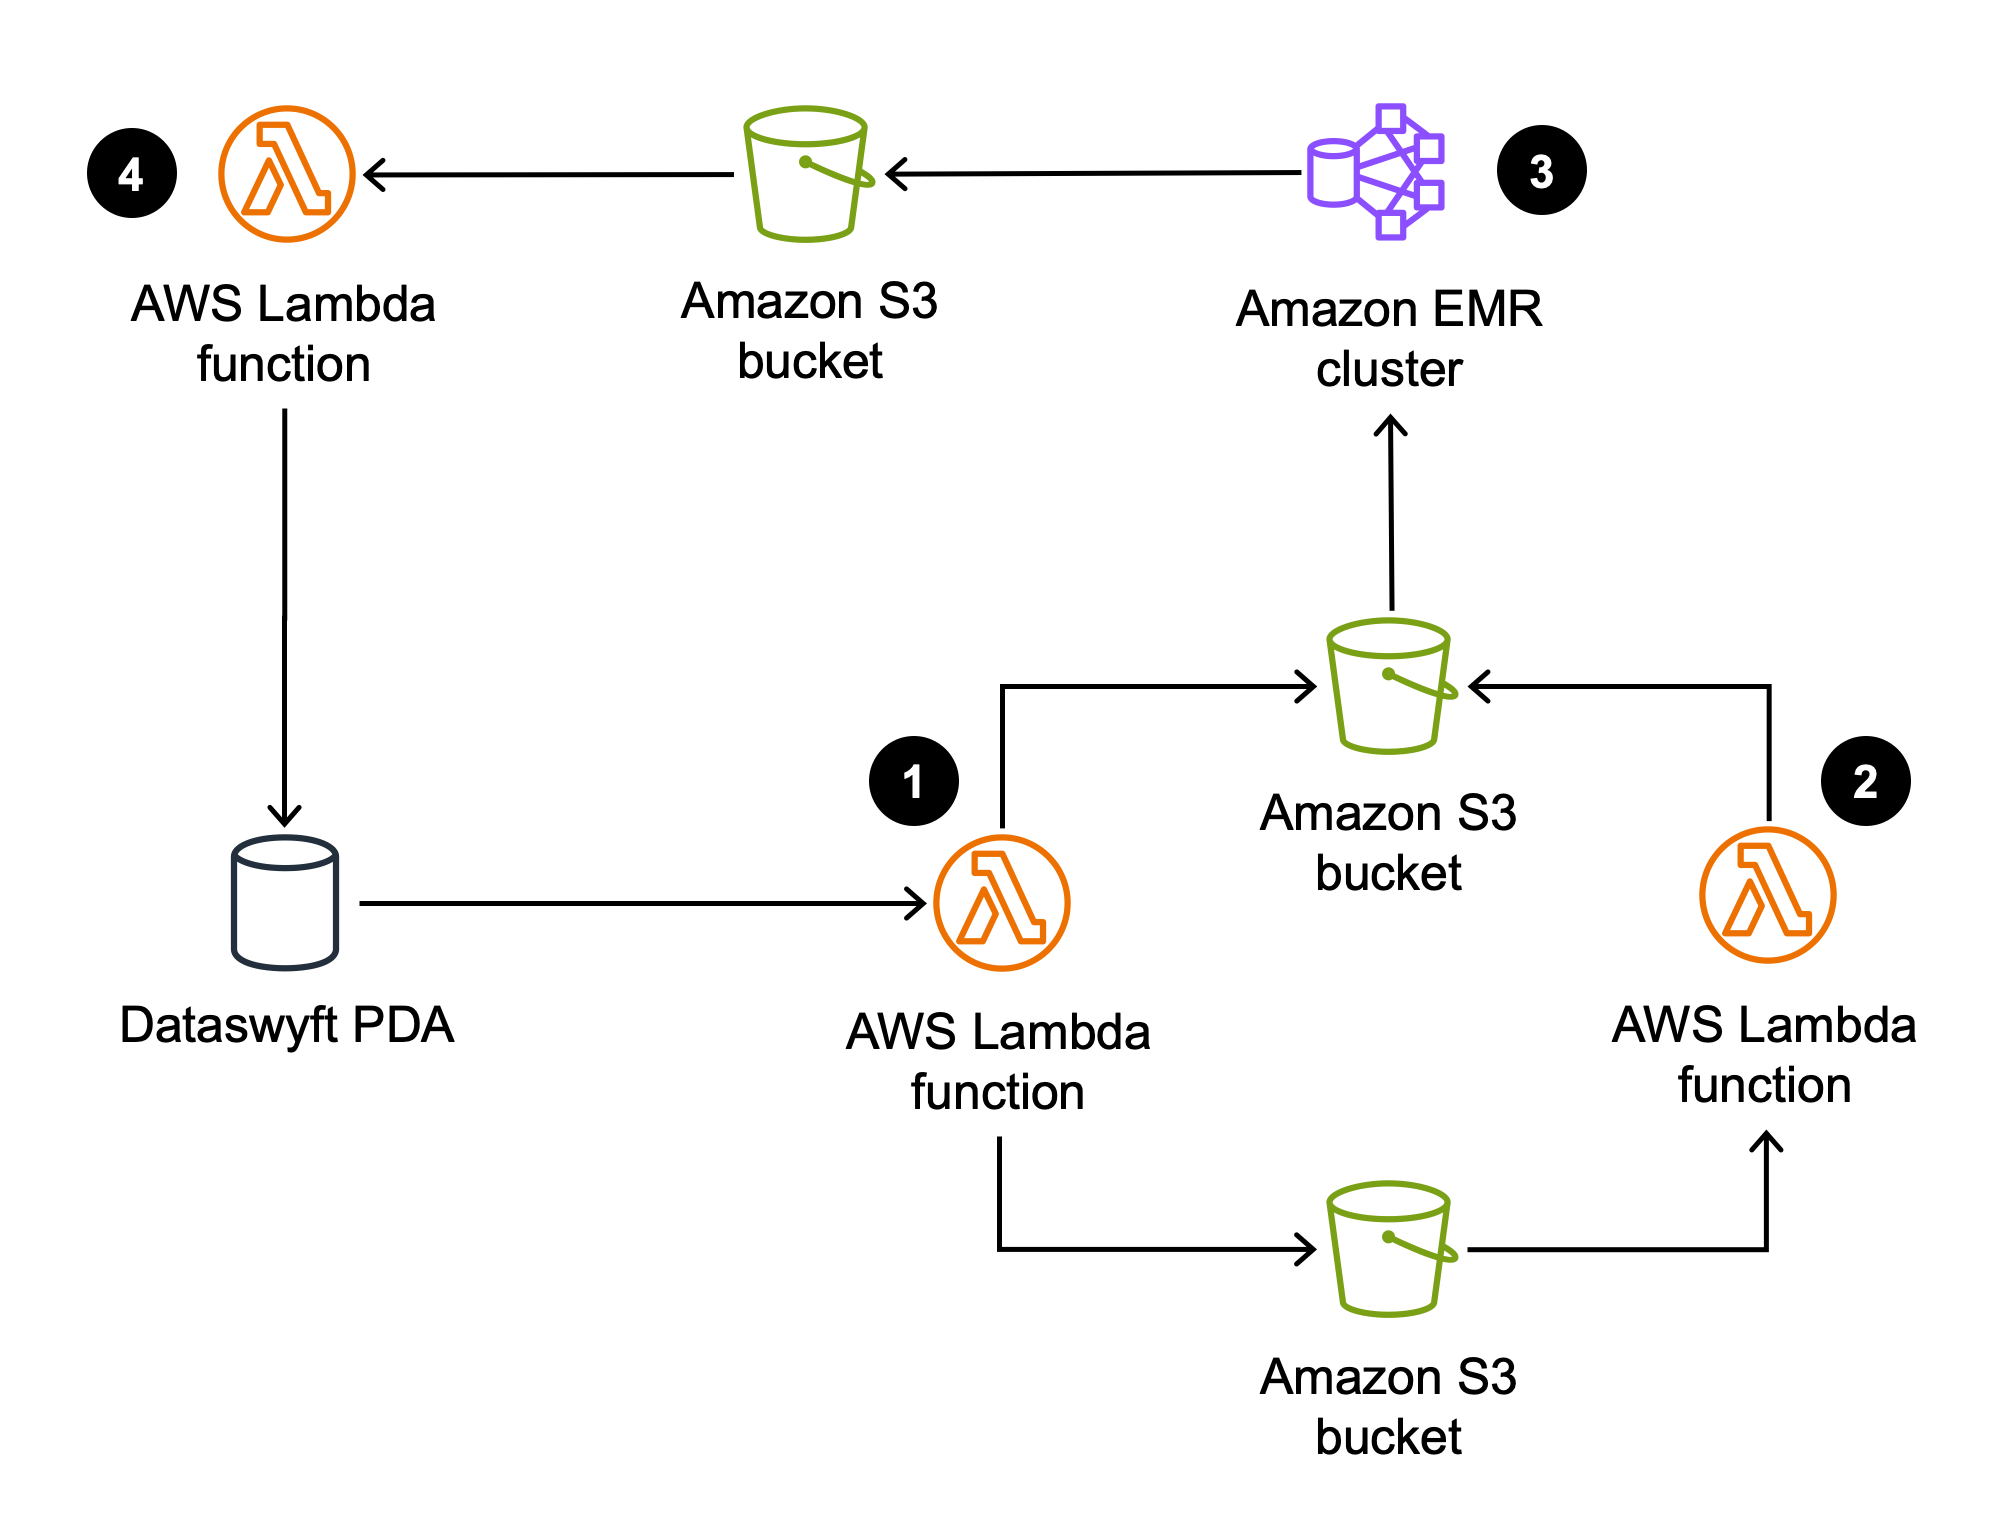
\includegraphics[width=\textwidth]{aws-architecture}
\caption[ShareTrace batch-processing architecture]{ShareTrace batch-processing architecture. \ding{202} An AWS Lambda function\protect\footnotemark{} retrieves the recent risk scores and location data from the Dataswyft Personal Data Accounts (PDAs) of ShareTrace users. Risk scores are formatted as Giraph \verticesName and stored in an Amazon Simple Storage Service\protect\footnotemark{} (S3) bucket. Location data is stored in a separate S3 bucket. \ding{203} A Lambda function performs a contact search over the location data and stores the contacts as Giraph edges in the same bucket that stores the Giraph \verticesName. \ding{204} Amazon Elastic MapReduce\protect\footnotemark{} (EMR) runs risk propagation as a Giraph job and stores the exposure scores in an S3 bucket. \ding{205} A Lambda function stores the exposure score of each user in their respective PDA.}
\label{fig:aws-architecture}
\end{figure}

\addtocounter{footnote}{-1}
\addtocounter{footnote}{-1}
\footnotetext[\thefootnote]{\url{https://aws.amazon.com/lambda}}
\addtocounter{footnote}{1}
\footnotetext[\thefootnote]{\url{https://aws.amazon.com/s3}}
\addtocounter{footnote}{1}
\footnotetext[\thefootnote]{\url{https://aws.amazon.com/emr}}

\clearpage

A couple factors prompted me to search for an alternative implementation.
  \begin{enumerate}
    \item \emph{Dependency management incompatibility}. The primary impetus for reimplementation was the dependency conflicts between Giraph and other libraries. Despite several attempts (e.g., using different library versions, using different versions of Giraph, and forcing specific versions of transitive dependencies) to resolve the conflicts, a lack of personal development experience and stalled progress prompted me pursue alternative implementations.
    \item \emph{Implementation complexity}. For a relatively straightforward data flow, the architecture in \cref{fig:aws-architecture} corresponded to over \num{4000} lines of source code. In retrospect, AWS Step Functions\footnote{\url{https://aws.amazon.com/step-functions}} could have been used to orchestrate the workflow, including the fan-out design pattern, which would have simplified the Lambda function implementations. Regarding the implementation of risk propagation, one-mode projection (first used in \cref{sec:projected-subgraphs}) would have simplified the implementation since it avoids multiple types of \verticesName and messages.
  \end{enumerate}

\section{Factor Subgraph Actors}\label{sec:subgraph-actors}

In an attempt to simplify the design in \cref{sec:giraph}, I rewrote risk propagation using the Ray Python library\footnote{\url{https://www.ray.io}}. While it claims to support actor-based programming, Ray only offers coarse-grained concurrency, with each actor being mapped to a physical core. To achieve parallelism, the factor graph was partitioned amongst the actors such that each actor maintained a subset of variable \verticesName \emph{or} factor \verticesName. The graph topology was stored in shared memory since it was immutable. The lifetime of this design was brief for the following reasons.
  \begin{enumerate}
    \item \emph{Poor performance}. Communication between Ray actors requires message serialization. Moreover, partitioning the factor graph into subsets of factor \verticesName and variable \verticesName results in maximal interprocess communication. Unsurprisingly, this choice of partitioning manifested in poor runtime performance.
    \item \emph{Design complexity}. Not using a framework, like Giraph, meant that this implementation required more low-level code to implement actor functionality and message passing. Regardless of the performance, the overall design of this implementation was poorly organized and overthought.
  \end{enumerate}

\section{Driver-Monitor-Worker Framework}\label{sec:dmw-framework}

Based on the poor runtime performance and complexity of the previous approach, I speculated that centralizing the mutable aspects of risk propagation (i.e., the iterative exposure scores of each variable \vertexName) would improve both metrics. With this is mind, I designed the \define{monitor-worker-driver} (DMW) \define{framework}, which draws inspiration from the \define{tree of actors} design pattern\footnote{\url{https://docs.ray.io/en/latest/ray-core/patterns/tree-of-actors.html}}. \Cref{fig:dmw-framework} describes the framework.

\begin{figure}[htbp]
\centering
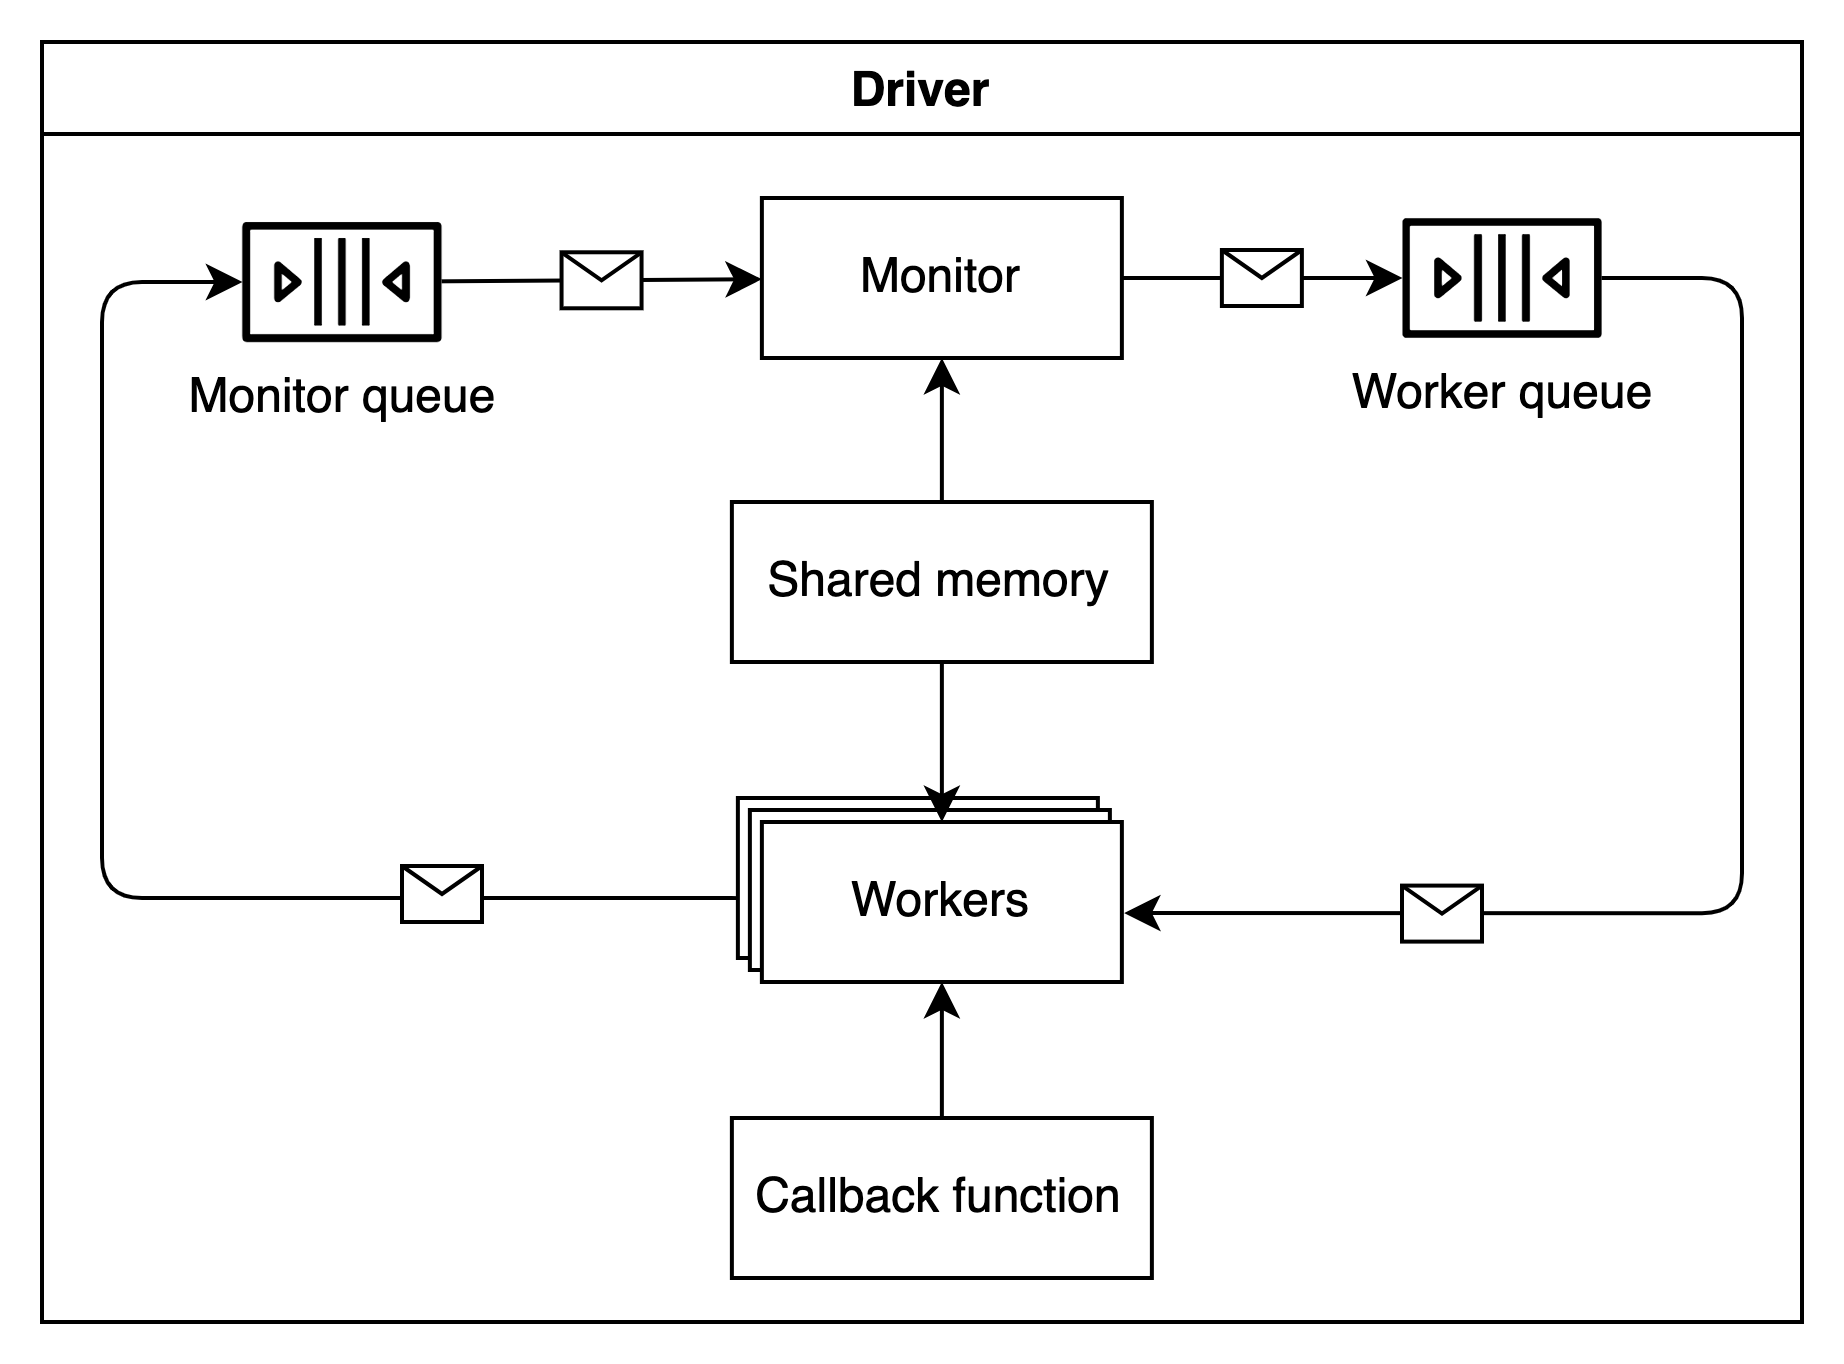
\includegraphics[width=\textwidth]{dmw-framework}
\caption[Driver-monitor-worker framework]{Driver-monitor-worker framework. The \define{driver} is the entry point into the program. It initializes the monitor and workers, and then waits for termination. The \define{monitor} encapsulates the mutable state of the program and decides which messages are processed by workers. A \define{worker} is a stateless entity that processes the messages that the monitor puts in the \define{worker queue}. Worker behavior is defined by a \define{callback function}, which typically depends on the message contents. The side effects of processing a message are recorded as new messages and put in the \define{monitor queue}. This cycle repeats until some termination condition is satisfied. Any immutable state of the program can be stored in \define{shared memory} for efficient access.}
\label{fig:dmw-framework}
\end{figure}

For risk propagation, the driver creates the factor graph from the set of risk scores $\vScores$ and contacts $\vContacts$, stores the factor graph in shared memory, sets the initial state of the monitor to be the maximum risk score of each individual, and puts all risk scores in the monitor queue. During message passing, the monitor maintains the exposure score for each variable \vertexName.

The DMW framework was the first approach that utilized the send coefficient to ensure the convergence and termination of message passing. However, because the DMW-based implementation assumed the factor graph representation of the contact network, the send coefficient was applied to both variable and factor messages.

Compared to \cref{sec:subgraph-actors}, this implementation provided a cleaner design and less communication overhead. However, what prompted yet another alternative implementation was its scalability. Because the monitor processes messages serially, it is a bottleneck for algorithms in which the workers perform fine-grained tasks. Indeed, the Ray documentation\footnote{\url{https://docs.ray.io/en/latest/ray-core/patterns/too-fine-grained-tasks.html}} notes that the parallelization of small tasks is an anti-pattern because the interprocess communication cost exceeds the benefit of multiprocessing. Unfortunately, the computation performed by factor \verticesName and variable \verticesName was fine-grained, so the scalability of the DMW framework was demonstrably poor.

\section{Projected Subgraph Actors}\label{sec:projected-subgraphs}

The last alternative design of risk propagation is the subject of published work \citep{Tatton2022b} and preprint \citep{Tatton2022a} which were written during the coarse of my graduate studies.

% Summary of approach

% Comparison to proposed approach in this work

% Summary of experimental results

%Like all previous designs, risk propagation is an offline algorithm. Let $\vGraph_i$ be \indexed{i}{subgraph of contacts} that is associated with \indexed{i}{actor}. It is assumed that actor communication is expensive, so a partitioning algorithm \citep{Buluc2016} that minimizes communication complexity between actors is key to maximizing performance. Each actor is associated with a \define{remote mailbox} and a \define{local mailbox}. The former is designated for messages sent by other actors, while the latter is designated for messages associated with individuals within the same subgraph. For an actor to send a message to another actor, it must know the address of the target actor's remote mailbox and an identifier of the individual within the target actor's subgraph. The \cRiskPropagationMain operation describes the main steps.

%Compared to asynchronous risk propagation (\cref{sec:asynchronous}), actor behavior differs in two significant ways:
%\begin{enumerate}
%  \item The send threshold is applied \emph{across} contacts and discriminates against risk scores that are newer than the initial exposure score $\dot{\vScore}_\vTime$. The latter is based on the assumption that newer risk scores are less likely to be propagated by other actors.
%  \item The initial risk score that is sent to each contact accounts for recency, which is assumed to exponentially decay with a rate constant of $\pRateConstant > 0$.

%%%%%%%%%%%%%%%%%%%

%The last alternative design of risk propagation is the subject of published work \citep{Tatton2022b} and preprint \citep{Tatton2022a}. Since those works were written during the coarse of my graduate studies, algorithmic details and experimental results are included below.

%\subsection{Risk Propagation}
%
%Like all previous designs, risk propagation is an offline algorithm. Let $\vGraph_i$ be \indexed{i}{subgraph of contacts} that is associated with \indexed{i}{actor}. It is assumed that actor communication is expensive, so a partitioning algorithm \citep{Buluc2016} that minimizes communication complexity between actors is key to maximizing performance. Each actor is associated with a \define{remote mailbox} and a \define{local mailbox}. The former is designated for messages sent by other actors, while the latter is designated for messages associated with individuals within the same subgraph. For an actor to send a message to another actor, it must know the address of the target actor's remote mailbox and an identifier of the individual within the target actor's subgraph. The \cRiskPropagationMain operation describes the main steps.
%
%\begin{function}{\nRiskPropagationMain}[\vScores, \vContacts]
%  \State $\vGraph \assign \cCreateContactNetwork[\vContacts]$
%  \ForEach{$i \in \intInterval{1}{n}$}
%    \State $\cRiskPropagationActor[\vGraph_i, \vScores_i]$
%  \EndFor
%  \State Collect the exposure scores from all actors
%\end{function}
%
%The \cRiskPropagationActor operation defines the behavior of an actor. According to \citet{Tatton2022a,Tatton2022b}, an actor terminates when no message has been received after a set period of time. \citet{Tatton2022a} also allows an actor to terminate after passing messages for a given duration; or if a certain number of messages have been received and none caused an individual's exposure score to be updated.
%
%\begin{function}{\nRiskPropagationActor}[\vGraph, \vScores]
%  \ForEach{$\vVertex_i \in \vVertices$}
%    \State $\tilde{\vScore}_{\vTime, i}, \dot{\vScore}_{\vTime, i}, \assign \max \vScores_i$
%    \ForEach{$\vVertex_j \in \vNeighbors_i$}
%      \State $\vScore_\vTime \assign \argmax \SetBuilder{\vScore_\vTime^{\pRateConstant(\vTime - \vTime_{ij})}}{\vScore_\vTime \in \vScores_i, \vTime < \vTime_{ij} + \pTimeBuffer}$
%      \State Send $\pTransmissionRate \vScore_\vTime$ to $\vVertex_j$
%    \EndFor
%  \EndFor
%  \While{termination condition is not satisfied}
%    \State Receive $\vScore_\vTime$ for $\vVertex_i$ from $\vVertex_j$
%    \State $\tilde{\vScore}_{\vTime, i} \assign \max \{\tilde{\vScore}_{\vTime, i}, \vScore_\vTime\}$
%    \ForEach{$\vVertex_k \in \vNeighbors_i \setminus \{\vVertex_j\}$}
%      \If{$\vTime < \vTime_{ik} + \pTimeBuffer$ \AND $\vScore_\vTime \geq \pSendCoefficient \dot{\vScore}_i$ \AND $\vTime \leq \dot{\vTime}_i$}
%        \State Send $\pTransmissionRate \vScore_\vTime$ to $\vVertex_k$
%      \EndIf
%    \EndFor
%  \EndWhile
%\end{function}
%
%Compared to asynchronous risk propagation (\cref{sec:asynchronous}), actor behavior differs in two significant ways:
%\begin{enumerate}
%  \item The send threshold is applied \emph{across} contacts and discriminates against risk scores that are newer than the initial exposure score $\dot{\vScore}_\vTime$. The latter is based on the assumption that newer risk scores are less likely to be propagated by other actors.
%  \item The initial risk score that is sent to each contact accounts for recency, which is assumed to exponentially decay with a rate constant of $\pRateConstant > 0$.
%\end{enumerate}
%As such, message reachability differs from \cref{eq:message-reachability}:
%\begin{equation}\label{eq:initial-message-reachability}
%  \vReachability(\vPath, \vMessage) = \sum_{(i, j) \in \vPath} [\pTransmissionRate^i \dot{\vScore}_\vSourceVertex \geq \pSendCoefficient \pTransmissionRate \dot{\vScore}_i] \cdot [\dot{\vTime}_\vSourceVertex \leq \dot{\vTime}_i] \cdot [\dot{\vTime}_\vSourceVertex < \vTime_{ij} + \pTimeBuffer],
%\end{equation}
%
%\subsection{Experiment Design}
%
%The following experiments were performed using the implementation of risk propagation available on GitHub\footnote{\url{https://github.com/cwru-xlab/sharetrace-ray}}:
%\begin{itemize}
%  \item \emph{Efficiency}. How does the transmission rate and send coefficient affect the runtime and number of messages sent during risk propagation? What is the optimal send coefficient for efficiency and accuracy?
%  \item \emph{Message reachability}. How accurately does \cref{eq:estimated-message-reachability} estimate \cref{eq:initial-message-reachability}?
%  \item \emph{Scalability}. How does the runtime of risk propagation relate to the size of the contact network?
%\end{itemize}
%\Cref{tab:appendix-experiments} summarizes the types of contact networks used for the experiments.
%
%\begin{table}[htbp]
%\centering
%\begin{tabular}{lccc}
%  \toprule
%  & Efficiency & Message reachability & Scalability \\
%  \midrule
%  Synthetic & \checkmark & \checkmark & \checkmark \\
%  Real-world & \checkmark & \checkmark & \\
%  \bottomrule
%\end{tabular}
%\caption[Experiments by contact network type]{Experiments by contact network type.}
%\label{tab:appendix-experiments}
%\end{table}
%
%The Case Western Reserve University high-performance computing cluster was utilized. For efficiency and message reachability experiments, \num{4} CPUs and \qty{8}{GB} memory were used. For scalability experiments, \numrange{8}{12} CPUs and \qtyrange{16}{64}{GB} memory were used. All experiments were run on a single cluster node.
%
%Unless stated otherwise, the transmission rate was $\pTransmissionRate = \num{0.8}$; the send coefficient was $\pSendCoefficient = \num{0.6}$; the time buffer was $\pTimeBuffer = \num{2}$ days; the risk score and contact expiries were $\pScoreExpiry = \pContactExpiry = \num{14}$ days; and the rate constant was $\pRateConstant = \num{1}$. Actors were configured to timeout after \num{3} seconds of not receiving any messages; or after receiving \num{10} times the number of individuals in messages that did not update an individual's exposure score.
%
%To partition the contact network, the METIS algorithm\footnote{\url{https://github.com/inducer/pymetis}} \citep{Karypis1998} was configured to use a load imbalance factor of \num{0.2}; to attempt contiguous partitions that have minimal inter-partition connectivity; to apply \num{10} iterations of refinement during each stage of the uncoarsening process; and to use the best of \num{3} cuts.
%
%Random geometric graphs [RGGs] \citep{Dall2002}, benchmark graphs [LFRGs] \citep{Lancichinetti2008}, and clustered scale-free graphs [CSFGs] \citep{Holme2002} were used as synthetic contact networks. Together, these graphs demonstrate aspects of community structure \citep{Fortunato2010}. When constructing RGGs, the radius was set to
%\begin{equation*}
%  r(n) = \min \{\num{1}, \num{0.25}^{\log_{10}(n) - 1}\},
%\end{equation*}
%where $n$ is the number of individuals. Used to construct LFRGs, a mixing parameter of $\mu = \num{0.1}$, a degree power-law exponent $\gamma = \num{3}$, a community size power-law exponent $\beta = \num{2}$, degree bounds $(k_\mathit{min}, k_\mathit{max}) = (\num{3}, \num{50})$, and community size bounds $(s_\mathit{min}, s_\mathit{max}) = (\num{10}, \num{100})$. These values are consistent with the recommendation to have $\gamma \in [\num{2}, \num{3}]$,  $\beta \in [\num{1}, \num{2}]$, $k_\mathit{min} < s_\mathit{min}$, and $k_\mathit{max} < s_\mathit{max}$ \citep{Lancichinetti2008}. When creating CSFGs, $m = \num{2}$ edges are added for each new \vertexName and a triad was formed with probability $P_t = \num{0.95}$. For all graphs, self-loops and isolated \verticesName are removed.
%
%Three real-world contact networks were used from the SocioPatterns project: a high school [Thiers13] \citep{Fournet2014}, a workplace [InVS15], and a scientific conference [SFHH] \citep{Genois2018}. Contact in these networks represents \num{20} seconds of face-to-face interaction. However, to remain consistent with risk propagation, only the most recent contact time was retained for each pair of individuals. \Cref{fig:real-networks} visualizes the contact network of each setting.
%
%\begin{figure}[htbp]
%\centering
%\subcaptionbox{Thiers13 (\num{180} \verticesName; \num{2220} edges)\label{fig:highschool12}}{
%  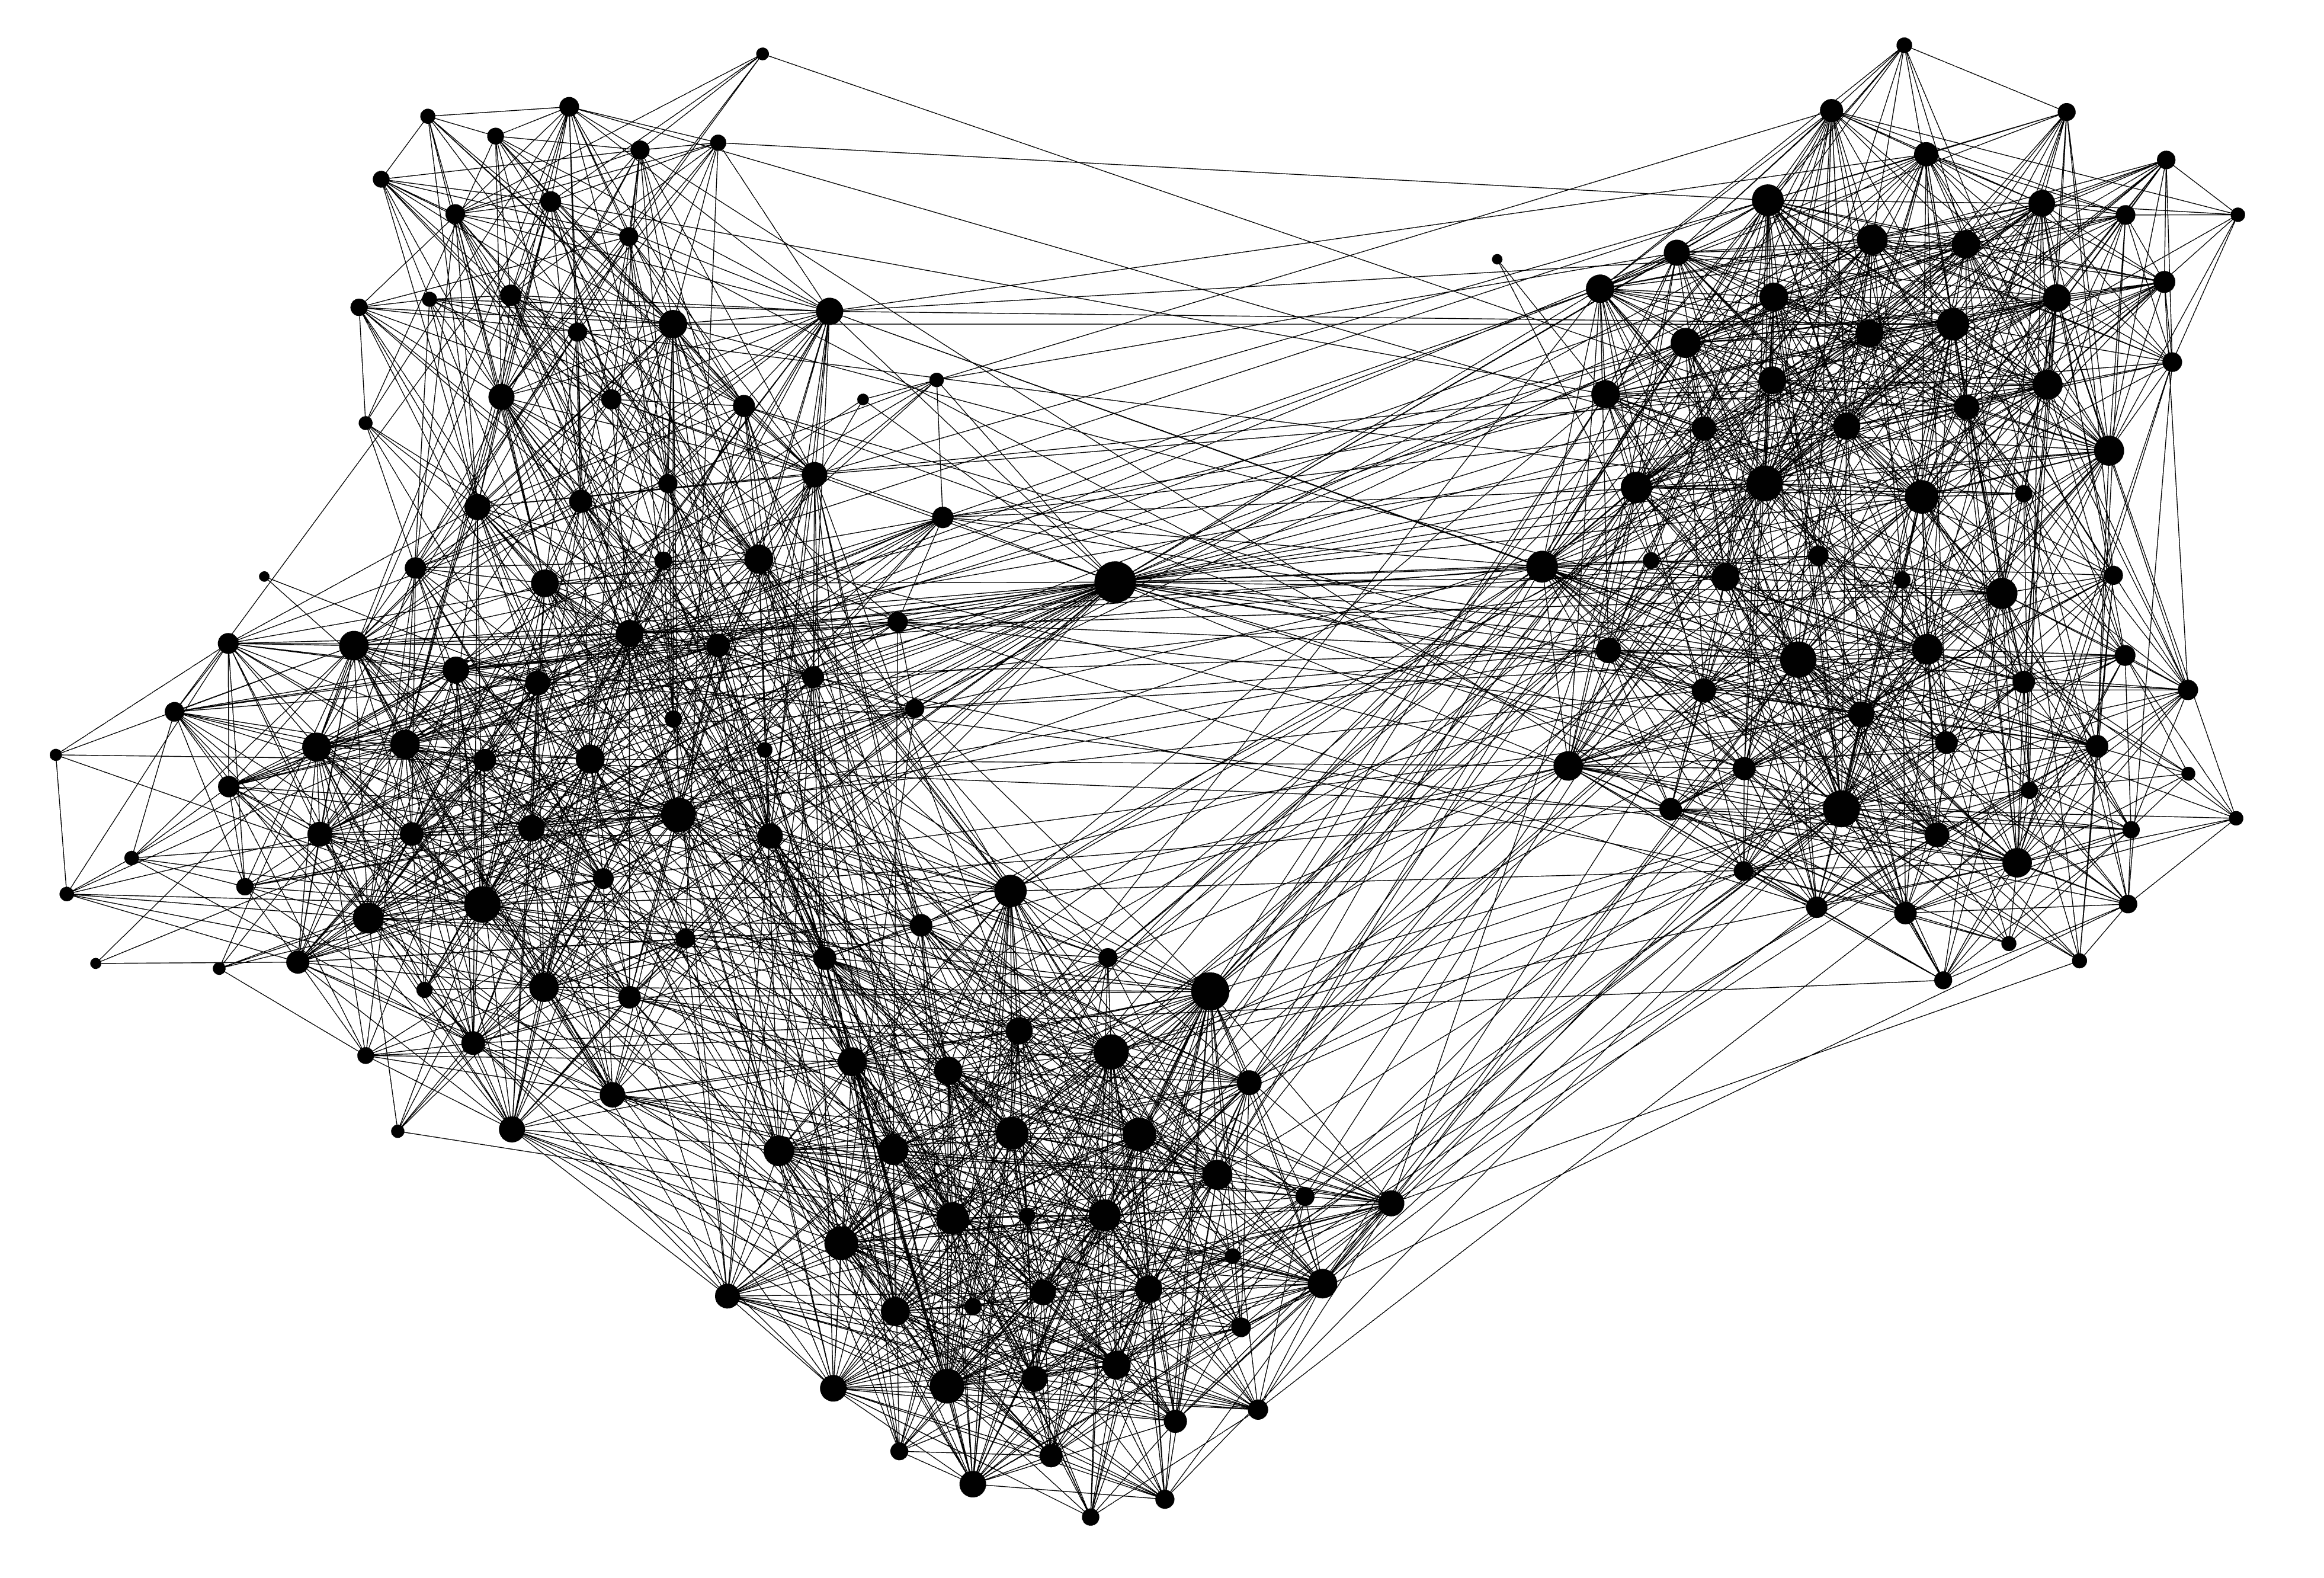
\includegraphics[height=0.275\textheight]{highschool12.png}
%}
%\subcaptionbox{InVS15 (\num{217} \verticesName; \num{4274} edges)\label{fig:workplace}}{
%  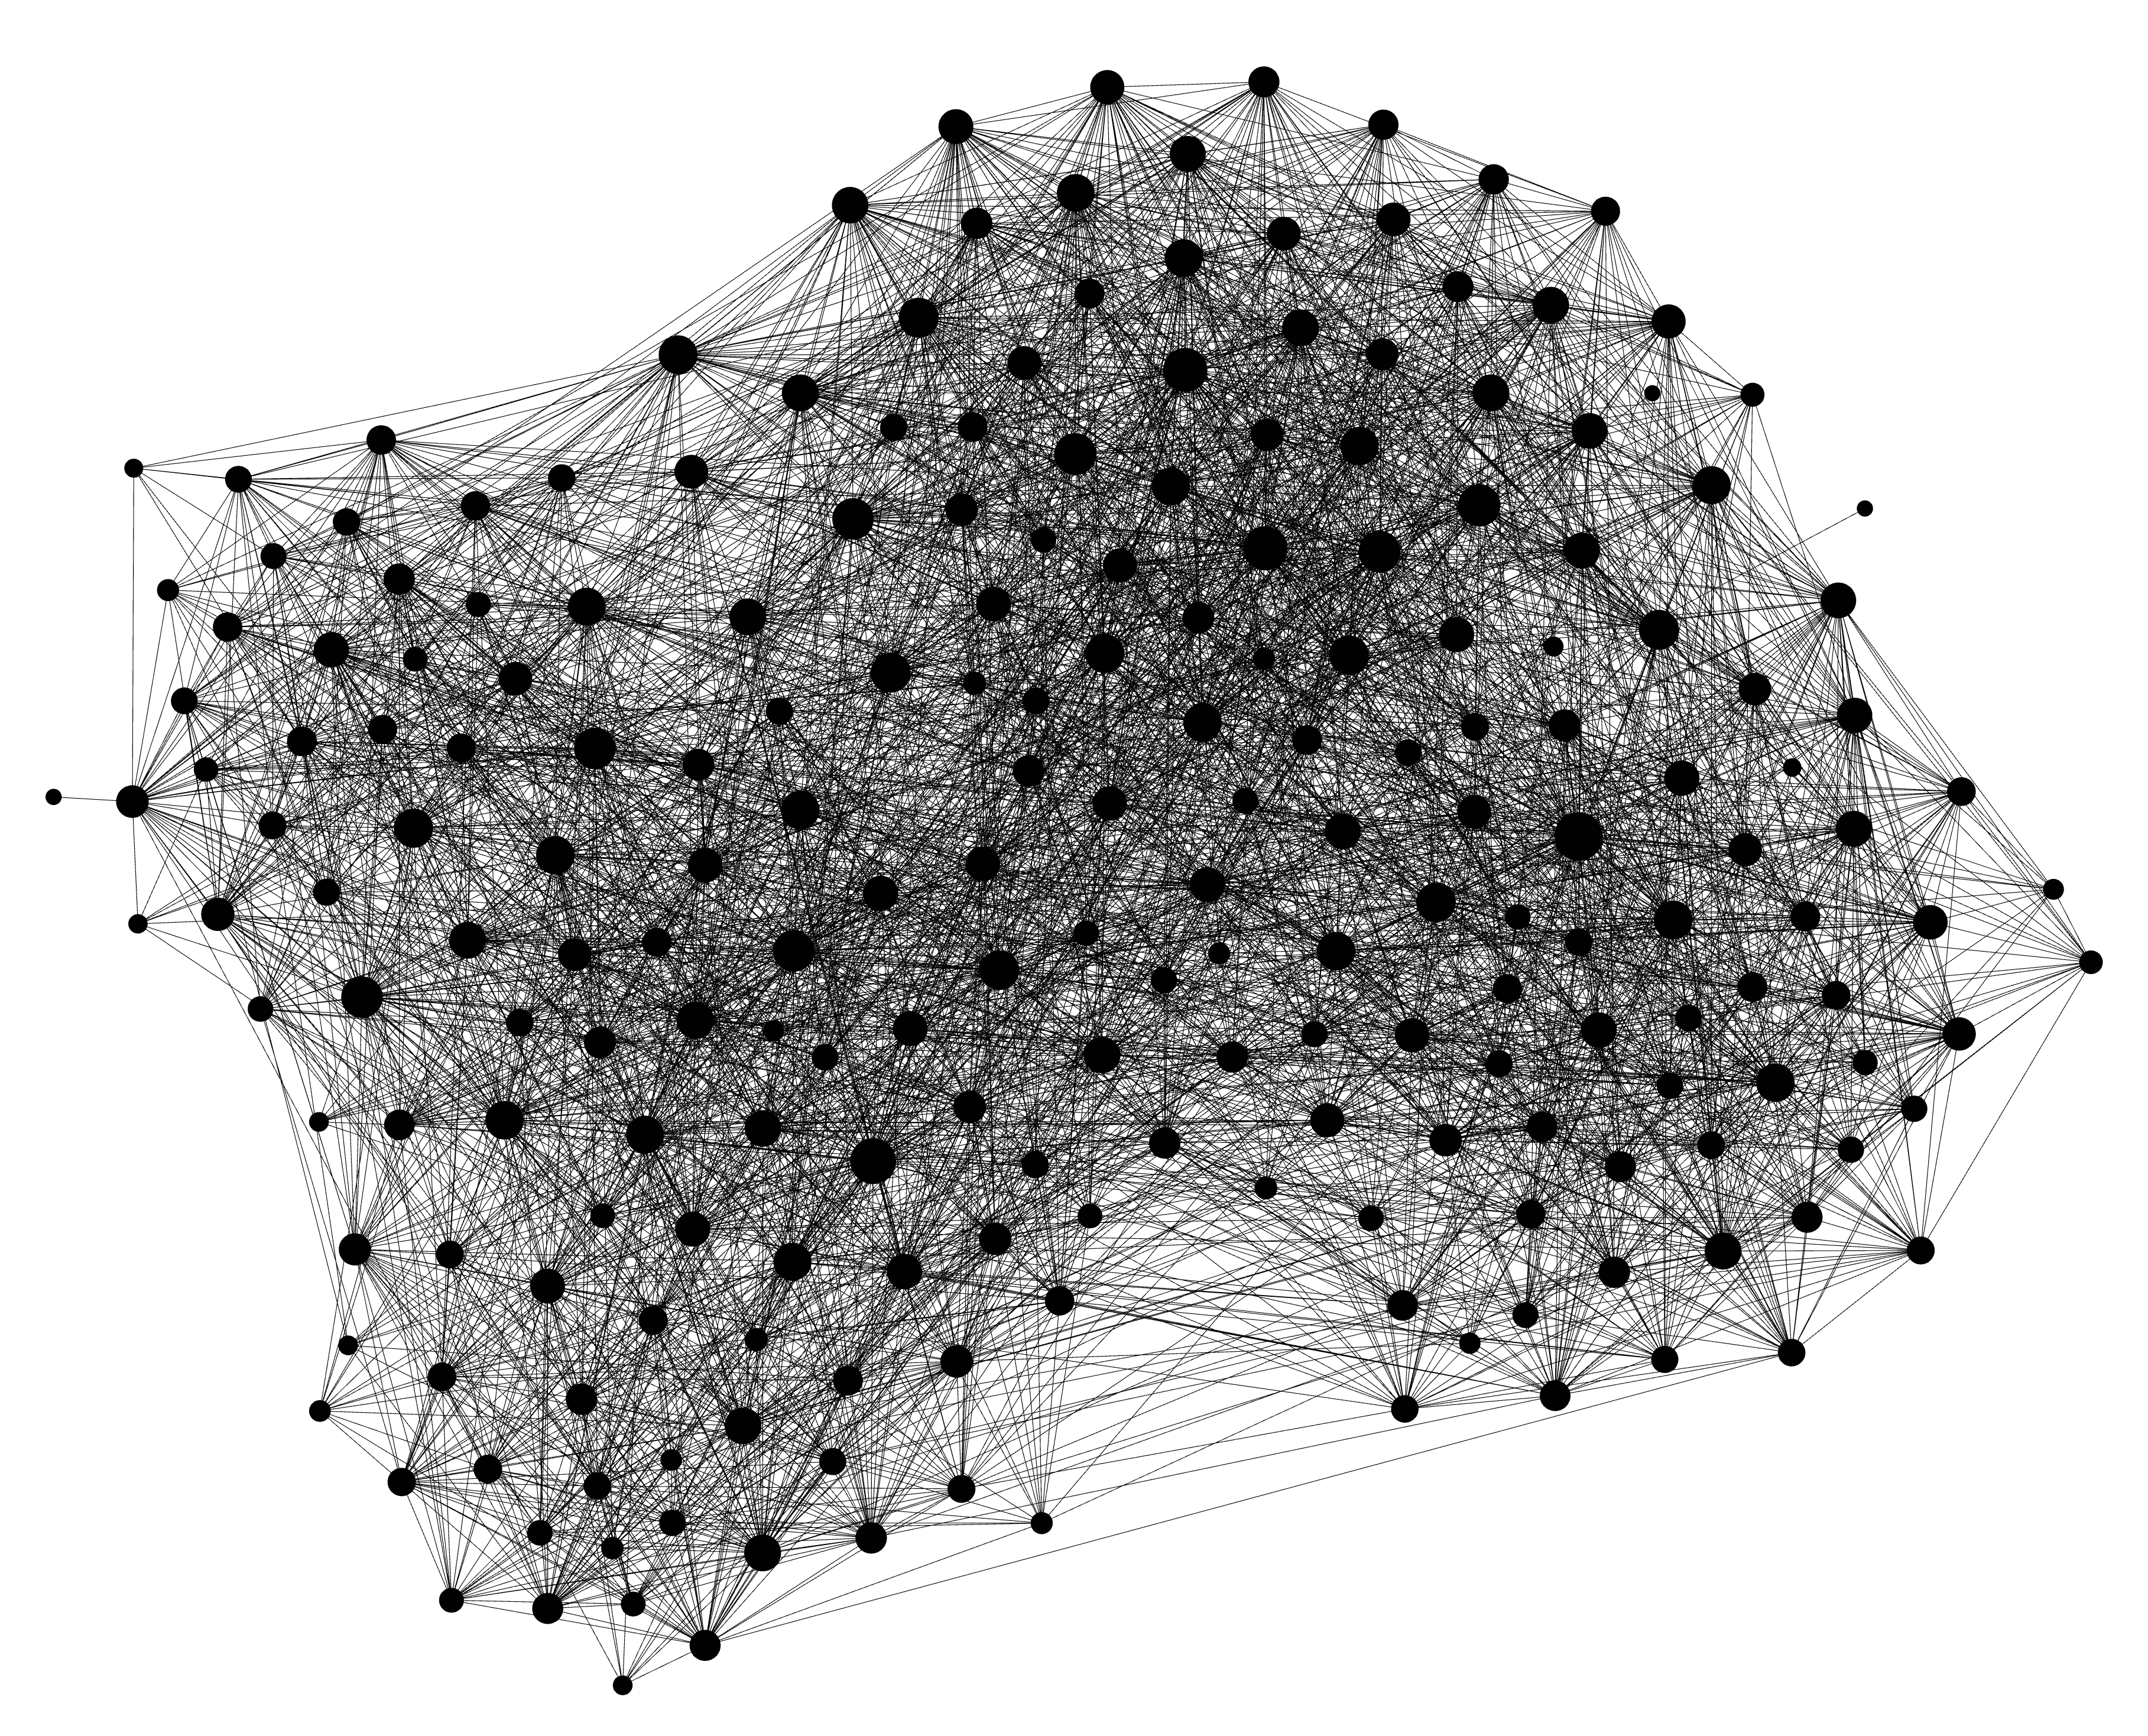
\includegraphics[height=0.275\textheight]{workplace.png}
%}
%\subcaptionbox{SFHH (\num{403} \verticesName; \num{9565} edges)\label{fig:conference}}{
%  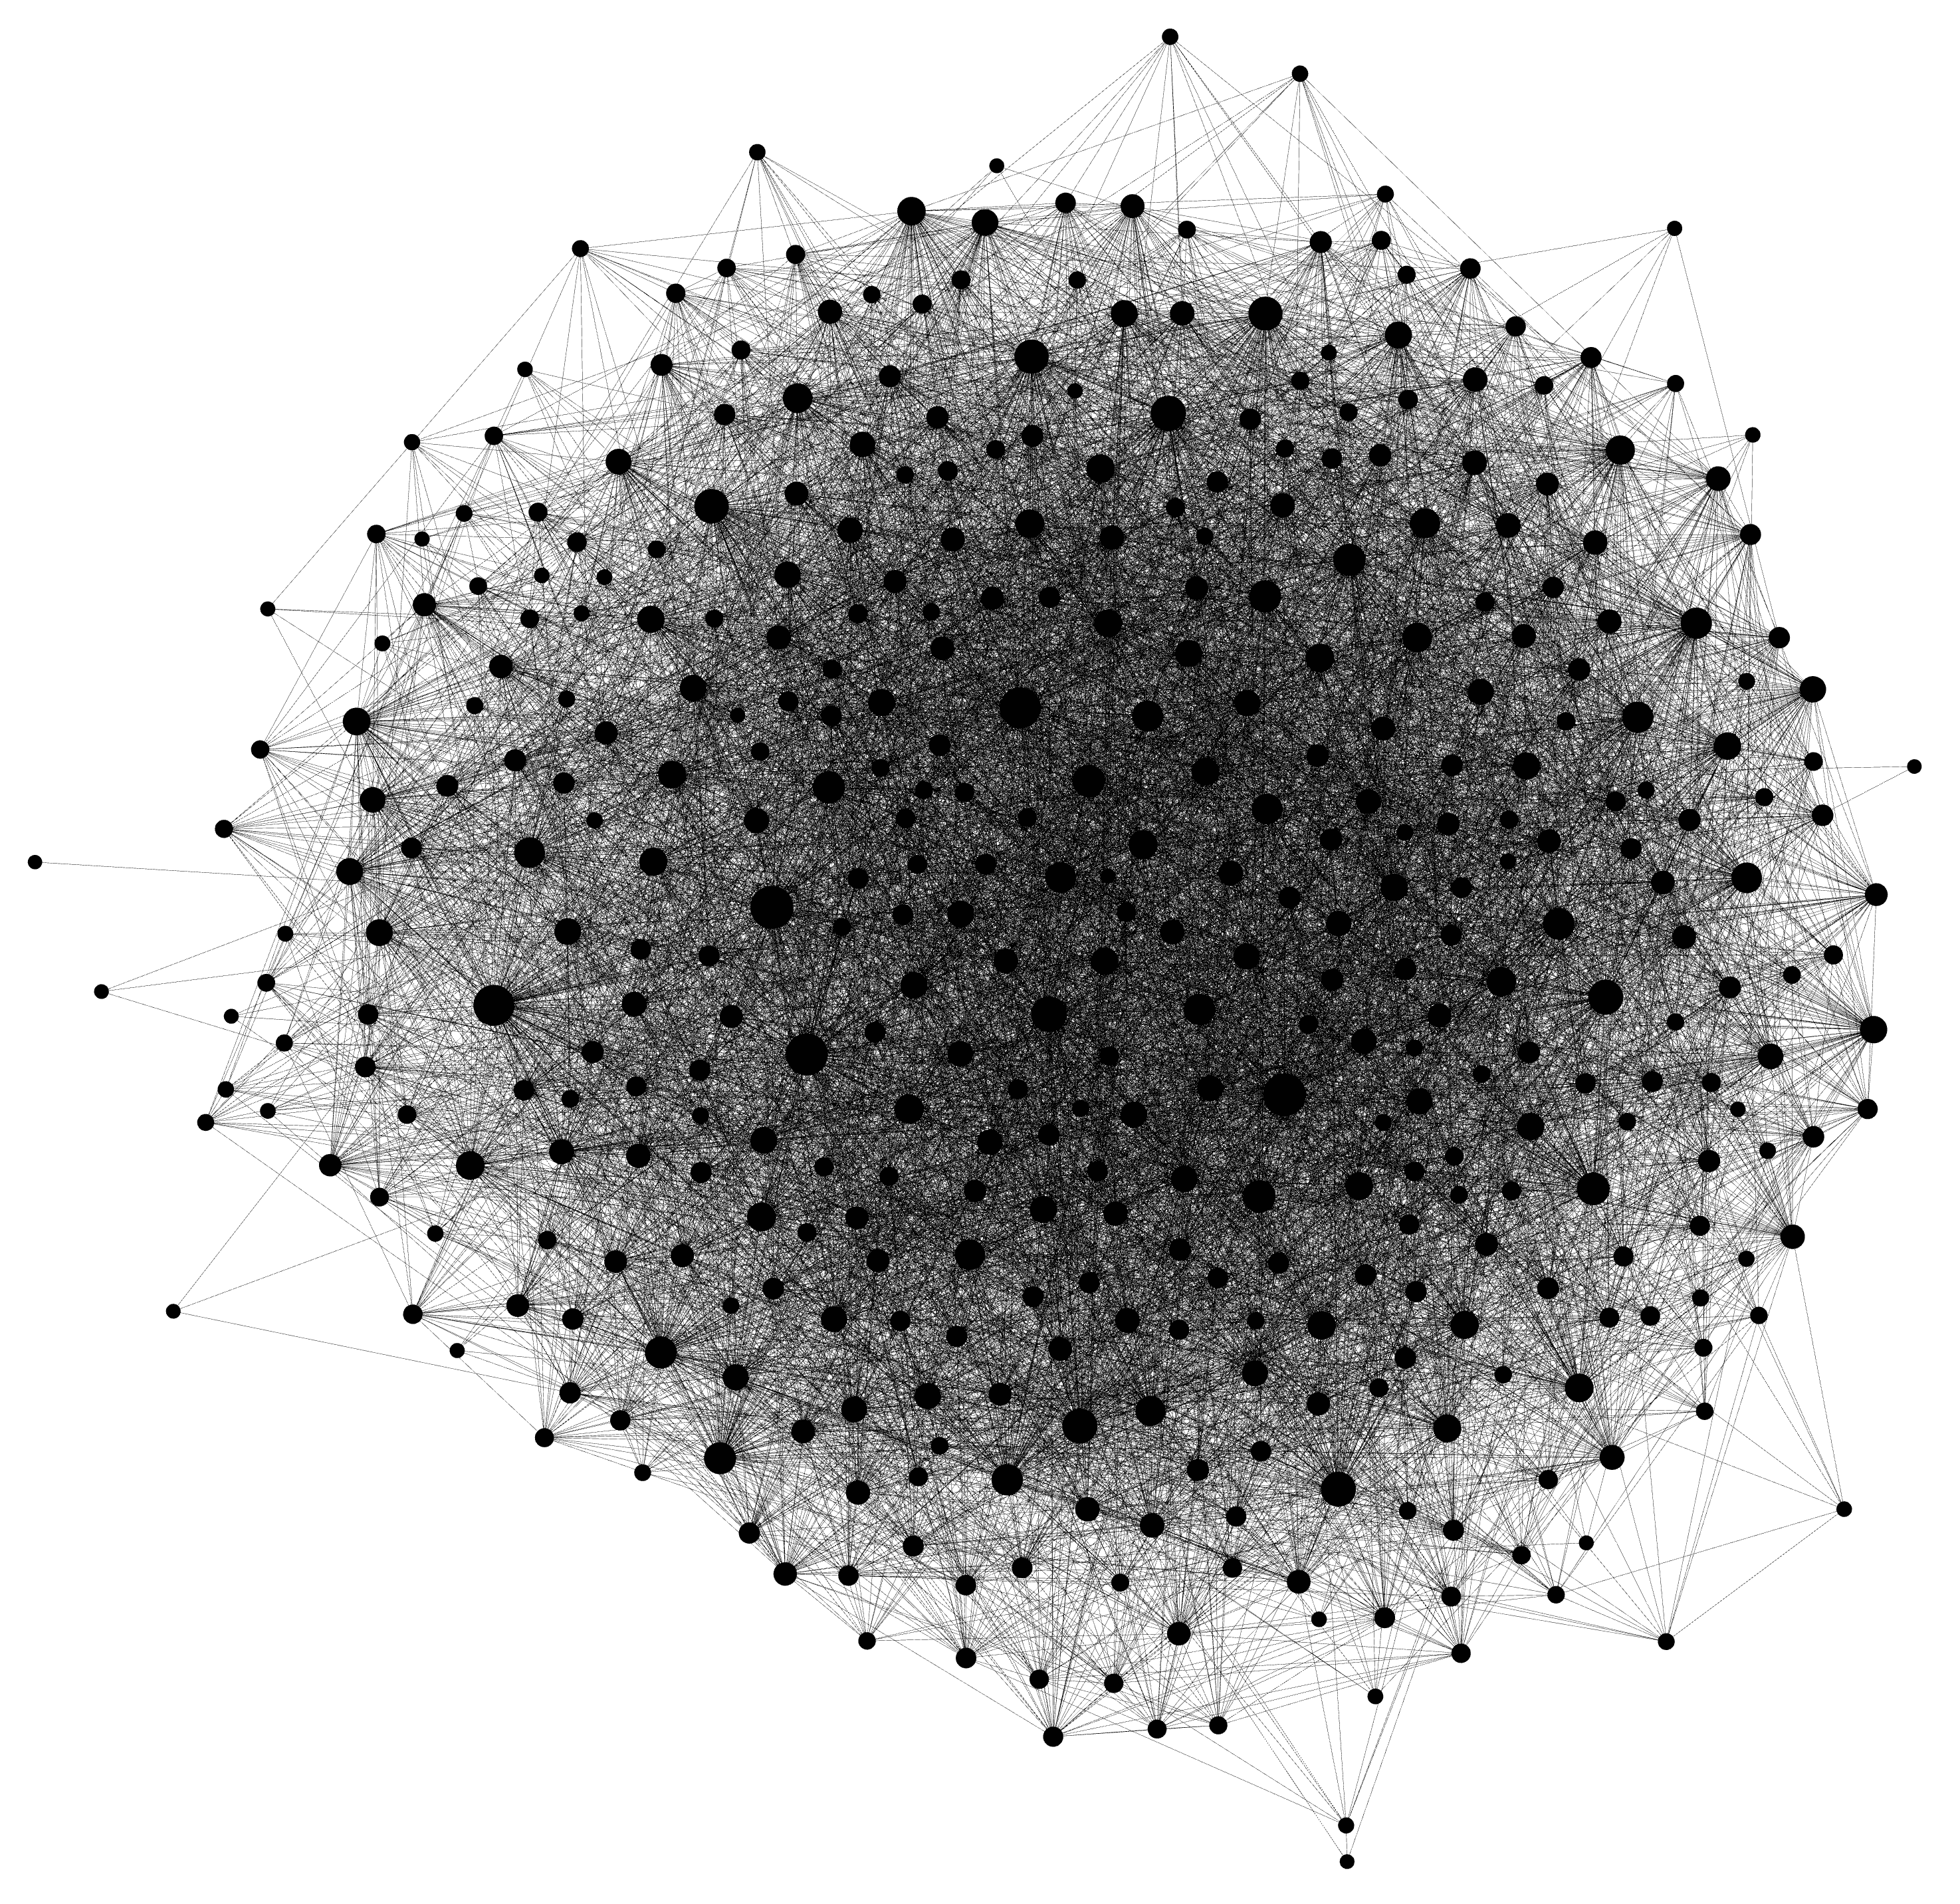
\includegraphics[height=0.275\textheight]{conference.png}
%}
%\caption{SocioPatterns contact networks}
%\label{fig:real-networks}
%\end{figure}
%
%The following defines the data generation process. Let $j \in \intInterval{0}{\pScoreExpiry}$ and $\delta_i \sim \uniformDistribution(\qty{0}{\second}, \qty{86400}{\second})$. Then the risk scores for \indexed{i}{individual} were
%\begin{equation*}
%  \vScores_i = 
%    \begin{cases}
%      \SetBuilder{\vScore_{\vTime_j} \sim \uniformDistribution(\num{0}, \num{0.5})}{ \vTime_j = \vReferenceTime + \delta_i + j \text{ days}} & \text{with probability } p = \num{0.8} \\
%      \SetBuilder{\vScore_{\vTime_j} \sim \uniformDistribution(\num{0.5}, \num{1})}{\vTime_j = \vReferenceTime + \delta_i + j \text{ days}} & \text{with probability } 1 - p.
%    \end{cases}
%\end{equation*}
%Contact times were similarly generated. For real-world contact networks, to ensure that all risk scores were initially propagated, the contact times were shifted forward by $\vReferenceTime$ and $\vReferenceTime - (1 \text{ day})$ was used for generating the timestamps of risk scores. In this way, the newest risk score was older than the oldest contact.
%
%To measure efficiency and message reachability, various transmission rates and send coefficients were evaluated:
%\begin{equation*}
%  (\pSendCoefficient, \pTransmissionRate) \in \{\num{0.1}, \num{0.2}, \ldots, \num{1}\} \times \{\num{0.1}, \num{0.2}, \ldots, \num{0.9}\}.
%\end{equation*}
%Synthetic contact networks of \num{5000} individuals and \num{2} subgraphs were used. For real-world contact networks, \num{10} iterations were performed over each data set to obtain an average performance.
%
%To measure the scalability of risk propagation, contact networks were generated with \numrange{100}{10000} individuals in increments of \num{100} and repeated for \num{10} iterations. No partitioning was performed for contact networks containing fewer than \num{1000} individuals; otherwise, \num{2} partitions were used. Additional partitioning did not improve performance due to interprocess communication\footnote{Clearly, \numrange{1}{2} partitions offers minimal parallelism. Limitations of the Ray library are suspected to be the cause of performance issues.}.
%
%\subsection{Experiment Results}
%
%\subsubsection{Efficiency}
%
%To determine accuracy, the maximum number of updates for a given transmission rate was used. \Cref{fig:efficiency} indicates that a send coefficient of $\pSendCoefficient = \num{0.6}$ achieved \qty{99}{\percent} accuracy. Beyond $\pSendCoefficient = \num{0.6}$, however, the transmission rate had considerable impact, independent of the contact network type.
%
%\Cref{fig:efficiency} shows a more variable relationship with respect to runtime and the number of messages. Generally, the transmission rate (resp., send coefficient) had a direct (resp., inverse) relationship with runtime and number of messages. However, LFRGs displayed less variability across send coefficients and transmission rates than RGGs and CSFGs. Therefore, it is useful to consider the lower quartile $Q_1$, the median $Q_2$, and the upper quartile $Q_3$, which shall be collectively reported as $(Q_1, Q_2, Q_3)$. For $\pTransmissionRate = \num{0.8} $ and $\pSendCoefficient = \num{0.6}$, risk propagation was more efficient with relative runtime $(\num{0.13}, \num{0.13}, \num{0.46})$ and relative number of messages $(0.13, 0.15, 0.44)$.
%
%\begin{figure}[htbp]
%\centering
%\begin{tikzpicture}
%\begin{groupplot}[
%  group style={
%    group size=1 by 3,
%    xlabels at=edge bottom,
%    ylabels at=edge left
%  },
%  boxplot,
%  table/col sep=comma,
%  boxplot/draw direction=y,
%  xtick distance=1,
%  scaled x ticks={base 10:-1},
%  width=\textwidth,
%  height=0.3\textheight,
%  ymin=-0.1,
%  xmin=0.25,
%  xmax=10.75,
%  ytick distance=0.2,
%  xtick scale label code/.code={},
%  xlabel={Send coefficient}
%  ]
%  \nextgroupplot[
%    table/y=NormalizedMessages,
%    ylabel={Number of messages}
%  ]
%  \foreach \t in {1,...,10} {
%    \addplot[color=black] table[only if={entry of SendTolerance is \t}]{tolerance-messages.csv};
%  }
%  \nextgroupplot[
%    table/y=NormalizedUpdates,
%    ylabel={Number of updates}
%  ]
%  \foreach \t in {1,...,10} {
%    \addplot[color=black] table[only if={entry of SendTolerance is \t}]{tolerance-updates.csv};
%  }
%  \nextgroupplot[
%    table/y=NormalizedRuntimeInSeconds,
%    ylabel={Runtime}
%  ]
%  \foreach \t in {1,...,10} {
%    \addplot[color=black] table[only if={entry of SendTolerance is \t}]{tolerance-runtime.csv};
%  }
%\end{groupplot}
%\end{tikzpicture}
%\caption[Parametric behavior of risk propagation efficiency]{Parametric behavior of risk propagation efficiency. All dependent variables are normalized across contact networks and transmission rates.}
%\label{fig:efficiency}
%\end{figure}
%
%\subsubsection{Message Reachability}
%
%Let the \define{actual/estimated message reachability ratio} be defined as
%\begin{equation*}
%  \text{A/E MRR} = \frac{\vReachability(\vPath, \vMessage)}{\vEstimatedReachability(\vPath)}.
%\end{equation*}
%
%Overall, \cref{eq:estimated-message-reachability} is a good estimator of \cref{eq:initial-message-reachability}. For synthetic networks, \cref{eq:estimated-message-reachability} underestimated \cref{eq:initial-message-reachability} with A/E MRR $(\num{0.71}, \num{0.84}, \num{0.98})$. For $\pTransmissionRate = \num{0.8}$ and $\pSendCoefficient = \num{0.6}$, the A/E MRR was $(\num{0.52}, \num{0.77}, \num{1.12})$ and $(\num{0.79}, \num{0.84}, \num{0.93})$, respectively. \Cref{tab:reachability} provides mean values of the A/E MRR for synthetic and real-world contact networks. \Cref{fig:ratio} indicates that moderate send coefficients tend toward more stable A/E MRRs. The A/E MRR tends to have an inverse relationship with the transmission rate.
%
%With a lower send coefficient and higher transmission rate, \cref{eq:estimated-message-reachability} suggests higher message reachability. However, because \cref{eq:estimated-message-reachability} does not account for the temporality constraints of message passing in risk propagation, \cref{eq:estimated-message-reachability} overestimates \cref{eq:initial-message-reachability}. While \cref{eq:estimated-message-reachability} is theoretically an upper bound on \cref{eq:initial-message-reachability}, it is possible for \cref{eq:estimated-message-reachability} to underestimate \cref{eq:initial-message-reachability} if the specified value of the initial risk score overestimates its actual value. When computing the A/E MRR for \cref{fig:ratio}, the mean initial risk score was used, so the A/E MRR is greater than \num{1} in some cases.
%
%\begin{figure}[htbp]
%\centering
%\begin{subfigure}[b]{\textwidth}
%\begin{tikzpicture}
%\begin{axis}[
%  boxplot,
%  table/col sep=comma,
%  boxplot/draw direction=y,
%  ylabel={A/E MRR},
%  xtick distance=5,
%  scaled x ticks={base 10:-1},
%  width=\textwidth,
%  height=0.35\textheight,
%  ytick distance=0.5,
%  xtick distance=1,
%  table/y=RatioValue,
%  xlabel={Send coefficient},
%  xmin=0.25,
%  xmax=10.75,
%  xtick scale label code/.code={}
%  ]
%  \foreach \t in {1,...,10} {
%    \addplot[color=black] table[only if={entry of SendTolerance is \t}]{ratio-tolerance.csv};
%  }
%\end{axis}
%\end{tikzpicture}
%\end{subfigure}	\\
%\begin{subfigure}[b]{\textwidth}
%\begin{tikzpicture}
%\begin{axis}[
%  boxplot,
%  table/col sep=comma,
%  boxplot/draw direction=y,
%  ylabel={A/E MRR},
%  xtick distance=5,
%  scaled x ticks={base 10:-1},
%  width=\textwidth,
%  height=0.35\textheight,
%  ytick distance=0.5,
%  xtick distance=1,
%  table/y=RatioValue,
%  xlabel={Transmission rate},
%  xmin=0.25,
%  xmax=9.75,
%  xtick scale label code/.code={}
%  ]
%  \foreach \t in {1,...,9} {
%    \addplot[color=black] table[only if={entry of Transmission is \t}]{ratio-transmission.csv};
%  }
%\end{axis}
%\end{tikzpicture}
%\end{subfigure}
%\caption[Parametric behavior of the A/E MRR]{Parametric behavior of the A/E MRR. Independent variables are grouped across contact networks.}
%\label{fig:ratio}
%\end{figure}
%
%\begin{table}[htbp]
%\centering
%\begin{tabular}{lS}
%  \toprule
%  Contact network & {A/E MRR $\pm$ \qty{95}{\percent} CI}\\
%  \midrule
%  \textit{Synthetic} & \num{0.85 \pm 0.08}\\
%  \tabindent LFR & \num{0.88 \pm 0.14}\\
%  \tabindent RGG & \num{0.74 \pm 0.12}\\
%  \tabindent CSFG & \num{0.90 \pm 0.14}\\
%  \midrule
%  \textit{Real-world} & \num{0.60 \pm 0.01}\\
%  \tabindent Thiers13 & \num{0.58 \pm 0.01}\\
%  \tabindent InVS15 & \num{0.63 \pm 0.01}\\
%  \tabindent SFHH & \num{0.60 \pm 0.01}\\
%  \bottomrule
%\end{tabular}
%\caption[Aggregate A/E MRRs by contact network]{Aggregate A/E MRRs by contact network, with transmission rate $\pTransmissionRate = \num{0.8}$ and send coefficient $\pSendCoefficient = \num{0.6}$. Ratios of synthetic contact networks are averaged across parameter combinations, while ratios for real-world contact networks are averaged across iterations.}
%\label{tab:reachability}
%\end{table}
%
%\subsubsection{Scalability}
%
%\Cref{fig:runtime} describes the runtime behavior of risk propagation. The runtime of CSFGs requires further investigation. A linear regression fit explains ($R^2 = \num{0.52}$) the runtime of LFRGs and RGGs with a slope $m = \num[exponent-mode=scientific]{0.0011 \pm 0.0001}$ and intercept $b = \num{4.3 \pm 1.6}$.
%
%\begin{figure}[htbp]
%\centering
%\begin{tikzpicture}
%\begin{axis}[
%  width=\textwidth,
%  height=0.3\textheight,
%  xlabel={Number of contacts},
%  ylabel={Runtime (\unit{\minute})},
%  ytick distance = 60,
%  scaled y ticks={real:60},
%  ytick scale label code/.code={}
%  ]
%  \addplot[
%    scatter,
%    only marks,
%    scatter src=explicit symbolic,
%    scatter/classes={1={mark=x,blue},2={mark=+,orange},3={mark=o,draw=green}},
%    mark size=2pt
%  ] table [col sep=comma,x=Edges,y=RuntimeInSeconds,meta=Graph]{scalability.csv};
%\legend{LFRG,CSFG,RGG}
%\end{axis}
%\end{tikzpicture}
%\caption[Risk propagation runtime]{Risk propagation runtime for contact networks containing \numrange{100}{10000} individuals and \numrange{200}{38000} contacts.}
%\label{fig:runtime}
%\end{figure}

\section{Contact Search}\label{sec:contact-search}

Though initial works on ShareTrace \citep{Ayday2020,Ayday2021} claim to use an individual's ephemeral identifiers to determine their contacts, this was practically infeasible at the time of development. As mentioned in \cref{sec:giraph}, the Exposure Notification API requires ephemeral identifiers to remain on an individual's mobile device. As such, I was tasked with devising an algorithm to find an individual's contacts based on their geolocation history; such an algorithm will be referred to as \define{contact search}. I ultimately discontinued this line of research in favor of the more scalable and privacy-preserving approach of ephemeral identifiers. Prior to this work, I was not familiar with computational geometry, nor the literature on the privacy-preserving extensions thereof. As such, the algorithms presented below are rudimentary and are not viable for practical usage.

Assume that \indexed{i}{individual's mobile device} maintains a history $\vLocations_i$ of their geolocation, such that $\vLocation_\vTime \in \vLocations_i$ represents the geolocation of \indexed{i}{location} at time $\vTime$. \Twoindexed{i}{j}{individuals} are \define{contacts} if the intersection of $\vLocations_i$ and $\vLocations_j$ contains a sequence of $\pProximity$-proximal geolocations over a $\pMinContactDuration$-contiguous time period (see \cref{sec:synchronous}). 

Assume an individual's geolocation history represents a piecewise constant function. That is, if $\vLocation_{\vTime_i}, \vLocation_{\vTime_k} \in \vLocations$, $\vLocation_{\vTime_j} \notin \vLocations$, and $\vTime_j \in [\vTime_i, \vTime_k)$, then $\vLocation_{\vTime_i} = \vLocation_{\vTime_j}$ and $\vLocation_{\vTime_j} \neq \vLocation_{\vTime_k}$. If $\pProximity = 0$, then the problem of deciding if \twoindexed{i}{j}{individuals} are contacts can be reduced to the longest common substring problem. Using piecewise constant interpolation such that $\vLocations_i$ and $\vLocations_j$ start and end at the same time, then each geolocation history represents a string, where the position of a character is the time at which the individual was at that location. If there exists a string of at least length $\pMinContactDuration$, then \twoindexed{i}{j}{individuals} are contacts. To find the most recent contact time, the two strings can be traversed in reverse order. Therefore, it takes time $\bigO{n^2}$ to find all contacts in a population of $n$ individuals. \Cref{fig:contact-search} provides a visual example of contact search.

\begin{figure}[htbp]
\centering
\begin{tikzpicture}[scale=2]
  \draw[latex-latex] (-3,0) -- (3,0);
  \draw[latex-latex] (-3, 1) -- (3,1);
  \draw (-2,0) -- (-2,1);
  \draw (-1.5,0) -- (-1.5,1);
  \draw (0.5,0) -- (0.5,1);
  \draw (2,0) -- (2,1);
  \draw (-1.75, 0.5) node {$A$};
  \draw (1.25, 0.5) node {$B$};

  \path [draw=black, fill=black] (-2,0) circle (1pt);
  \path [draw=black, fill=black] (0,0) circle (1pt);
  \path [draw=black, fill=black] (2,0) circle (1pt);
  \path [draw=black, fill=black] (-2.5,1) circle (1pt);
  \path [draw=black, fill=black] (-1.5,1) circle (1pt);
  \path [draw=black, fill=black] (0.5,1) circle (1pt);
  \path [draw=black, fill=black] (2.5,1) circle (1pt);
  
  \node[below=2pt of {(-2,0)}] {$\vLocation_2$};
  \node[below=2pt of {(0,0)}] {$\vLocation_6''$};
  \node[below=2pt of {(2,0)}] {$\vLocation_{10}'$};
  \node[above=2pt of {(-2.5,1)}] {$\vLocation_1$};
  \node[above=2pt of {(-1.5,1)}] {$\vLocation_3'$};
  \node[above=2pt of {(0.5,1)}] {$\vLocation_7''$};
  \node[above=2pt of {(2.5,1)}] {$\vLocation_{11}$};
\end{tikzpicture}
\caption[Example of contact search]{Example of contact search. Each line denotes time, increasing from left to right. A point $\vLocation_i$ is a geolocation that is recorded at time $i$. Regions $A$ and $B$ indicate periods of time in which the two individuals were colocated, but, for the sake of example, only region $B$ represents contact (e.g., $\pMinContactDuration > 1$).}
\label{fig:contact-search}
\end{figure}

The same string algorithm can be applied when $\pProximity > 0$ if geolocations are encoded to represent regions of space. One such encoding is \define{geohashing}, which transforms \define{geographic coordinates} (i.e., latitude-longitude ordered pairs \citep[p. 5]{Sickle2004}) into alphanumeric strings, called \define{geohashes}, where the length of a geohash correlates with its geospatial precision \citep{Morton1966}. This encoding obfuscates an individual's precise location, which provides some basic privacy. However, obfuscation can quickly lead to dense contact networks, which adversely impacts the accuracy and performance of an offline implementation of risk propagation.

Another approach to solving contact search when $\pProximity > 0$ is to construct a spatial data structure, such as a ball tree \citep{Omohundro1989, Kibriya2007}, from the geolocations of all individuals. To find an individual's contacts, a fixed-radius near neighbors search \citep{Bentley1975, Brin1995} can performed for each geolocation in the individual's history. Additional bookkeeping is needed to determine which individuals correspond to the neighbors of a geolocation. 

Any metric can be paired with a ball tree. However, because geolocations are represented as geographic coordinates, metrics that assume a Cartesian coordinate system may be unsuitable. The simplest geometric models of the Earth is that of a sphere. Given two geographic coordinates, the problem of finding the length of the geodesic\footnote{The \define{geodesic} is the shortest segment between two points on an ellipsoid \citep{Lu2014}.} between them is known as the \define{inverse geodetic problem} \citep{Sjoberg2012}. Assuming a spherical Earth, the solution to the inverse problem is to find the length of the segment that joins the two points on a great circle\footnote{The \define{great circle} is the cross-section of a sphere that contains its center \citep{Lu2014}}.

Let $\vAngle = \frac{\dist}{\vRadius}$ be the \define{central angle}, where $\dist$ is the distance between the two points along the great circle of a sphere with radius $\vRadius$ (see \cref{fig:central-angle}).

\begin{figure}[htbp]
\centering
\begin{tikzpicture}
  \def\myrad{2.25cm} % radius
  \def\myang{60} % arc angle
  \coordinate (O) at (0,0); % origin
  \draw (O) % circle and the dot at the origin
    node[circle,inner sep=1.5pt,fill] {} circle [radius=\myrad];
  \draw % θ arc
    (\myrad,0) coordinate (xcoord) --
    node[midway,below] {$\vRadius$} (O) --
    (\myang:\myrad) coordinate (slcoord)
    pic [draw,angle radius=1cm,"$\vAngle$"] {angle = xcoord--O--slcoord};
  \draw[|-|] % outer arc
    (\myrad+10pt,0)
    arc[start angle=0,end angle=\myang,radius=\myrad+10pt] 
    node[midway,fill=white] {$\dist$};
\end{tikzpicture}
\caption[Central angle of a great circle]{Central angle of a great circle.}
\label{fig:central-angle}
\end{figure}

The \define{haversine} (i.e., the half ``versed'' sine) of a central angle $\vAngle$ is defined as
\begin{equation}
  \hav \theta = \frac{\vers \theta}{2}  = \frac{1 - \cos \theta}{2}= \sin^2 \frac{\theta}{2}.\label{eq:hav}
\end{equation}
The great-circle distance $\dist$ between two points can be found by inversing \cref{eq:hav} and solving,
\begin{equation*}
  \dist(\vLocation, \vLocation') = 2 \cdot \arcsin \sqrt{\hav \frac{\vLatitude - \vLatitude'}{2} + \cos \vLatitude \cdot \cos \vLatitude' \cdot \hav \frac{\vLongitude - \vLongitude'}{2}},
\end{equation*}
where $\vLocation = (\vLatitude, \vLongitude)$ is a latitude-longitude coordinate in radians \citep[pp. 157--162]{Brummelen2013}.

More advanced \define{geodetic datum} \citep[pp. 71--130]{Lu2014} could be used to provide better geospatial accuracy. Additionally, by projecting geodetic coordinates onto the plane, metrics that assume a Cartesian coordinate system could be used instead \citep[pp. 265--326]{Lu2014}.